
\documentclass{article}

\usepackage{amsmath}
\usepackage{amssymb,amsmath}\usepackage{graphicx}\usepackage{hyperref}
\newcounter{prob}\setcounter{prob}{1}\newcommand{\prob}{\arabic{prob}.\indent \addtocounter{prob}{1}}

\newenvironment{amatrix}[1]{%
	\left(\begin{array}{@{}*{#1}{c}|c@{}}
	}{%
\end{array}\right)
}
\renewcommand{\thesubsection}{\Roman{subsection}}
\title{Group Project 1}
\date{02-19-2017}
\author{Frankington, Frank\\Stefanin, Annick\\Talada, Jeffrey\\Klobas, Anthony\\ Tran, Kevin\\  }
\begin{document}
\pagenumbering{gobble}
\maketitle
\newpage
\pagenumbering{arabic}

\section{Part 1}
First we will write out a few examples to see if any patterns emerge starting at our base case 8 cents worth of stamps, the smallest amount that can be made up using a three cent stamp and a five cent stamp. Intuitively, there should at least be a pattern that cycles over 15 steps as there might be $3×5$ different combinations.

\begin{table}[h]
	\caption{Stamp Values}
	\centering
	\begin{tabular}{c rrrrrrrrrrrrrrr}
		\hline\hline
		Total stamp value & 8 & 9 & 10 & 11 & 12 & 13 & 14 & 15 & 16 & 17 & 18 & 19 & 20 & 21 & 22 \\[0.5ex]
	\hline
	3 cent stamps & 1 & 3 & 0 & 2 & 4 & 1 & 3 & 0 & 2 & 4 & 1 & 3 & 0 & 2 & 4\\
	5 cent stamps & 1 & 0 & 2 & 1 & 0 & 2 & 1 & 3 & 2 & 1 & 3 & 2 & 4 & 3 & 2\\ [1ex] % [1ex]
	\hline
\end{tabular}
\label{tab:hresult}
\end{table}

\begin{itemize}
	\item First we can see that there are possible combinations of stamps for all amounts up to twenty-two cents.
	\item Second, from the examples we can see two different patterns, a cycle of three and a cycle of five. Because there are surjective cycles, we can conclude that indeed, we can produce any amount greater than or equal to eight cents from a combination of three cent and five cent stamps.
	\item We can choose the cycle of three to minimize use of five cent stamps or the cycle of five to minimize both three cent stamps and overall number of stamps. We will show this later.
\end{itemize}

\noindent Let S(an) = F(an) + T(an) for n = 8  (finds total number of stamps)

\noindent F(an) = F(an–5) + 1; (finds number of five cent stamps)

With base cases: F(8) = 1; F(9) = 0; F(10) = 2; F(11) = 1; F(12) = 0

\noindent T(an) = T(an–5);       (finds number of three cent stamps)

With base cases: T(8) = 1; T(9) = 3; T(10) = 0; T(11) = 2; T(12) = 4
\newpage
\section{Part 2}
\paragraph{Suppose $x+\frac{1}{x}$ is an integer. Prove by induction that $x^n + \frac{1}{x^n}$ for every $n\geq1$ would also be an integer. }
\paragraph{Before we start, let us note that we assume that $x$ is a valid value in order for instances of $x + \frac{1}{x}$ to yield a defined integer. We have also chosen to re-represent the problem using the recurrence relation that we found: $a_{n+1} = a_{n}*a_{1}-a_{n-1}$  with $a_{0}=2$ and $a_{1}=x+\frac{1}{x}$}. 
\paragraph{For the first base case: If $n=1$, then $a_{1}=x^{n=1} + \frac{1}{x^{n=1}} = x + \frac{1}{x}$; an integer. }
\paragraph{For the second base case, let us consider the case when $n = 2$. If $n = 2$, then $a_{n=2}=a_{1}^2-a_{0}$, which is $(x+\frac{1}{x})^2-2$, expanded as: $x^2 + \frac{1}{x^2}+2-2$. Notice that $(x^2 + \frac{1}{x^2} +2)$ is $a_{1}^2$ so we can rewrite the expanded form further as $a_{1}^2 = a_{2} + 2$ or $a_{2} = a_{1}^2 - 2$. Since the first base case is an integer, an $integer^2 + 2$ or $integer * integer + 2$ will result an integer. }

\paragraph{We will now prove the hypothesis by induction, showing that $a_{n+1}$ (when $n=n+1$) is also an integer. }
\begin{itemize}
	\item{$a_{n+1}=a_{n} * a_{1} -a_{n-1}$, so $a_{n+1}=(x^n + \frac{1}{x^n}) * (x + \frac{1}{x})-(x^{n-1} + \frac{1}{x^{n-1}})$}
	\item{We expand the first part to get}
	\item{$a_{n+1}=(x^{n+1}+\frac{1}{x^{n+1}})+(x^{n-1}+\frac{1}{x^{n-1}})-(x^{n-1} + \frac{1}{x^{n-1}})=(x^{n+1}+\frac{1}{x^{n+1}})$}
	\item{ we see that$(x^{n+1}+\frac{1}{x^{n+1}})$ is in fact the closed form for $a_{n+1}$ so we have show our inductive hypothesis to be true} 
	\item{Testing for $a_{2}$, $a_{1+1} = a_{1}*a_{1}-a_{0}$. $a_{0}$ = $x^0 + \frac{1}{x^0}$ = 2 when the $x$ values result in an integer. This is equivalent to an $integer*integer-2$; which results in an integer. }
	\item{Then for every increment of $a_{n}$, it will always calculate an $integer*integer-integer$, resulting in an integer. }
\end{itemize}
\paragraph{Thus, if $x + \frac{1}{x}$ is an integer then  $x^n + \frac{1}{x^n}$ is an integer, for every $\textit{n}\geq1$. }

\newpage
\section{Part 3}

Write a proof that all positive integers $\ge 2$ are either prime or can be written as the product of primes.\vspace{0.5in}

There are two conditions:

\prob Assume $k$ is a prime, no further work needs to be done.

\prob Assume $k$ is a non-prime $\in \mathbb{N}$

$a$ and $b \in \mathbb{N}$

$k = ab$ where $1 \leq a, b, < k$\\


For our Base Case $k = 2$

2 is a prime, and therefore fulfills our first condition.\\

Thus:

For the purpose of the proof we will assume these statements are true up through $n$. Using induction we shall prove it holds true for $n+1$.

If $n+1$ is a prime it fulfills the first condition, and therefore the theorem holds true.

If $n+1$ is not a prime it can be written as $(n+1) = ab$ where $1 \leq a, b, < (n+1)$

As both $a$ and $b < n$, they fall under the previous proof and prove our theorem.

So, $a$ can be written as: $a = p_1p_2p_3.......p_h$ and $b$ can be written as $b = q_1q_2q_3.......q_i$ , products of primes.

\paragraph{Thus, either a number $k \in \mathbb{N}$ is a prime, or it can be written as a product of primes: $n = ab$,  $n = p_1q_1....p_hq_i$. }

\newpage
\section{Part 4}

a. Show your work to solve the recurrence relation $$a_n= \frac{1}{2}a_{n-1}+\frac{7}{2}a_{n-2}-3a_{n-3}\ ; \ a_0=3,\ a_1=-5,\ a_2=\frac{29}{2}$$\\

We start by defining a function $S(a_n) =a_{n+1}$, This function is linear\footnote{Proof of this is beyond the scope of this problem} and we apply it as such:
$$S^3(a_{n-3})= \frac{1}{2}S^2(a_{n-3})+\frac{7}{2}S(a_{n-3})-3a_{n-3}$$\\
we then factor out $a_{n-3}$ \footnote{dark magic}
$$S^3= \frac{1}{2}S^2+\frac{7}{2}S-3$$
$$S^3 -\frac{1}{2}S^2-\frac{7}{2}S+3=0$$
$$\frac{1}{2}(S-1)(S+2)(2S+3)=0$$
We now know the closed form is of the form:
$$a(1)^n+b(-2)^n+c(\frac{3}{2})^n$$
We now substitute $n=0;n=1;n=2$ to create a system of equations to find a b and c
$$\begin{amatrix}{3}
	1 & 1 & 1 & 3 \\  1 & -2 & \frac{3}{2} & -5 \\ 1 & 4 & \frac{9}{4} & \frac{29}{2} 
\end{amatrix}$$
$$\begin{amatrix}{3}
1 & 0 & 0 & -2 \\  0 & 1 & 0 & 3 \\ 0 & 0 & 1 & 2 
\end{amatrix}$$
So we now believe the closed form is:
$$-2(1)^n+3(-2)^n+2(\frac{3}{2})^n$$
When testing the base cases $\ a_0=3,\ a_1=-5,\ a_2=\frac{29}{2}$
We now test by the Inductive Hypothesis that if every element of the recurrence is substituted with the closed form it should be consistent for the $n+1$th element\\
our recurrence is:
$$a_{n+1}= \frac{1}{2}a_{n}+\frac{7}{2}a_{n-1}-3a_{n-2}$$
So our I.H. produces:
$$-2(1)^{n+1}+3(-2)^{n+1}+2(\frac{3}{2})^{n+1}=$$$$ \frac{1}{2}(-2(1)^{n}+3(-2)^{n}+2(\frac{3}{2})^{n})+\frac{7}{2}(-2(1)^{n-1}+3(-2)^{n-1}+2(\frac{3}{2})^{n-1})-3(-2(1)^{n-2}+3(-2)^{n-2}+2(\frac{3}{2})^{n-2})$$
pulling down exponents we see:
$$-2-24(-2)^{n-2}+\frac{27}{4}(\frac{3}{2})^{n-2}=$$$$ \frac{1}{2}(-2+12(-2)^{n-2}+\frac{9}{2}(\frac{3}{2})^{n-2})+\frac{7}{2}(-2-6(-2)^{n-2}+3(\frac{3}{2})^{n-2})-3(-2(1)^{n-2}+3(-2)^{n-2}+2(\frac{3}{2})^{n-2})$$
We now seperate and group by the bases/powers:
$$-2-24(-2)^{n-2}+\frac{27}{4}(\frac{3}{2})^{n-2}=(-1-7+6) +(6-21-9)(-2)^{n-2}+(\frac{9}{4}+\frac{21}{2}-6)(\frac{3}{2})^{n-2}$$
simplifying yields: 
$$-2-24(-2)^{n-2}+\frac{27}{4}(\frac{3}{2})^{n-2}=-2 -24(-2)^{n-2} +\frac{27}{4}(\frac{3}{2})^{n-2}$$

We have thus proven by I.H. that our closed form will work for any $a_n$ where $n\geq0$\\


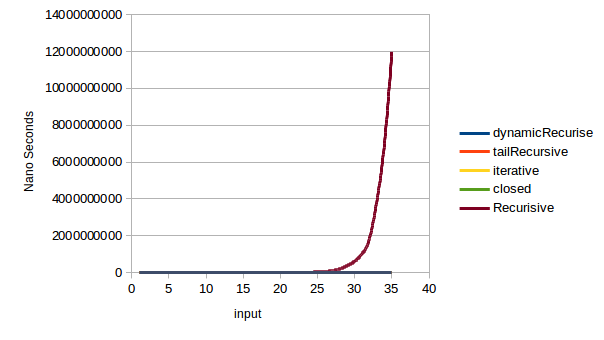
\includegraphics{Exponential.png}
Here we see the naive recursive function runs in exponential time which crushes everything else. so lets look at these data without the recursive function\\

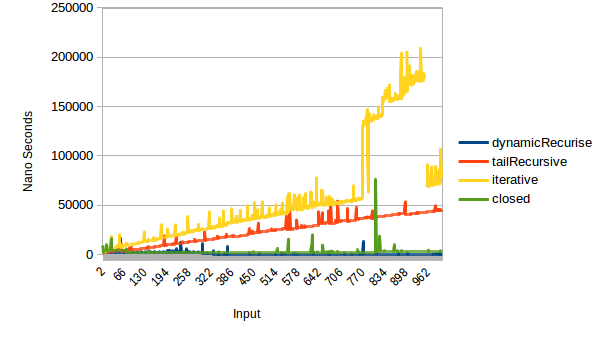
\includegraphics{FastTest.png}
iterative and tail recursive both run in what appears to be linear time. through the iterative one takes much more time after 700, this is most likely due to my choice of data structure


\newpage
\section{Part 5}
The following claim is clearly incorrect:\\

{\bf Claim:} If $n$ is an even number and $n\ge 2$, then $n$ is a power of two.\\

{\bf ``Proof":} We proceed by induction on the even number $n$. \\

Base Case: When $n=2$, $n=2^1$, a power of two.\\

Inductive Step: We will assume that for all even integers $k$ less than the nexteven number $n$, $k$ is a power of 2.  Using this assumption we will show that $n$ is also a power of $2$.\\

Since $n$ is even (and indeed at least 4), there is some $2\le k<n$ so that $n=2\cdot k$.  By the inductive hypothesis, $k$ is a power of two ($k=2^p$ for some $p$), and hence $n$ is $2\cdot 2^p=2^{p+1}$.  \\

Conclusion: We have shown that previous even integers being powers of two guarantees that the next even integer will also be a power of two.  Since the base case is verified, this constitutes a proof by induction that all even integers $\ge 2$ are powers of two.\\

%answer
\paragraph{Specifying that there is a $k$ such that $2=k<n$ and $2·k=n$ doesn’t guarantee that $k$ is even and therefore, might not be a power of two, only that $n$ is even. Hence, the recurrence relation can’t be properly established.}
\newpage
\section{Part 6}
(a)  If players 1-10 play the game when the jerseys numbered 1-10 are placed in lockers 1-10 in the order (from locker 1 to 10):
$$3-2-6-8-1-9-10-4-5-7$$

(i) The sequence of 5 lockers player one opens:
$$1-3-6-9-5$$

(ii) The cycles present in this permutation are:
$$1-3-6-9-5$$
$$2$$
$$4-8$$
$$7-10$$

(iii) The players will win on this arrangement of lockers. The longest cycle is length 5.

(iv) The players will fail with this arrangement:
$$2-3-4-5-6-7-8-9-10-1$$
They will will with this arrangement:
$$2-3-4-5-1-7-8-9-10-6$$


(b) Every cycle is closed: there is nothing that points to any part of the cycle that is not in the cycle. This is because there is only 1 of each pointer and by  definition the n-1th locker in the cycle points to locker n so it must have that pointer.

Every player starts by opening the locker with their own number and so if they loop, they will eventually be pointed at their own number and thus win. Everyone opens 5 lockers so if every $cycle \leq 5$ then everyone wins.

If a $cycle \geq 6$ exists then every player on that cycle will not loop, and 
thus have not seen the number of the locker they started with(their own) and thus will not win the game.\\

(c) The probability of losing for a team of 8 players = $\frac{1}{5}+\frac{1}{6}+\frac{1}{7}+\frac{1}{8}=\frac{533}{840}$
the probability of winning =1-prob of loss = $\frac{307}{840}$\\

(d) probability\footnote{seems like it should be easy to compute, but kept second guessing} that does not contain a $cycle \geq \frac{1}{3}$ 


\end{document}
